Cosys-AirSim's architecture is driven by a robust system of specialized classes. This section examines these core components. The fundamental distinction within this architecture is the division of labor: AirLib serves as a standalone C++ library responsible for the mathematical, engine-agnostic simulation logic, while the Unreal Engine plugin manages the 3D environment rendering, collision detection, and user interface.

\subsubsection{AirLib: The Simulation Core}
\noindent
AirLib core components include:

\begin{description}
    \item[\texttt{AirSimSettings}:] It parses the \texttt{settings.json} file, defines the configuration data structures (e.g., for vehicles, their type or initial spawn positions/orientations), manages default fallbacks when information is omitted, and operates as a globally accessible singleton.
    It defines ten vehicle types, acting as a pre-packaged combination of the physical body, the physics engine, and the firmware interface, and supports four simulation modes (i.e., multirotor, car, skid vehicle and computer vision).
    \item[Physics engine:]  This is a header-only physics engine. It is designed to be fast and extensible to implement different vehicles. It calculates forces, torques, velocities, and accelerations for the vehicles. It receives collision data from the Unreal Engine wrapper and calculates the resulting physical response (e.g., bouncing or crashing).
    \texttt{\seqsplit{FastPhysicsEngine}} updates the exact position and orientation of the vehicles at extremely high frequencies. It handles physics for drones; while for cars, the simulation relies entirely on Unreal Engine (\texttt{Chaos} \texttt{Physics} in UE5). On the other hand, \texttt{\seqsplit{ExternalPhysicsEngine}} allows the drone to be controlled via \texttt{\seqsplit{setVehiclePose()}}, keeping the drone in place until the next call. It is especially useful for moving the drone using an external simulator or on a saved path.
    \item[Sensor models:] These are header-only models for \textbf{sensors}. While Unreal Engine renders the visual data for cameras, AirLib handles the mathematical simulation of non-visual sensors. It takes the "Ground Truth" data from the physics engine and applies realistic noise, drift, and physics principles to generate sensor readings. Sensors include IMUs, LiDARs, GPS and others.
    \item[Control library:] This component provides an abstract base class for APIs and concrete implementations for platforms like MavLink. It enables programmatic control via Python and C++. AirLib operates an RPC server (default port 41451), while the \texttt{ApiProvider} routes incoming commands to the appropriate vehicle instance.
    \item[Clocks:] AirLib utilizes custom clocks to manage simulation time. The \texttt{ScalableClock} allows the simulation to run faster or slower than real-time, while the \texttt{SteppableClock} decouples simulation time from wall-clock time, advancing only in discrete steps upon command.
    \item[Firmware:] Multirotor and car \textbf{firmware} acts as the vehicle's controllers. It takes high-level commands (like "fly to 50 meters"), reads the simulated sensor data, and runs complex control loops to output the exact parameters needed to execute that command.
          \texttt{\seqsplit{SimpleFlight}} is AirSim's custom, built-in flight controller. Other open-source controllers are supported, such as \texttt{\seqsplit{ArduCopter}} and \texttt{\seqsplit{PX4}} for drones and \texttt{\seqsplit{ArduRover}} for cars.
\end{description}

\subsubsection{Unreal Engine: The Rendering and Interaction Layer}
\noindent
The Unreal Engine plugin transposes AirLib's logic into a 3D environment.
\begin{description}
    \item[\texttt{ASimHUD}:]  The core class responsible for the Head-Up Display (HUD), handling the visual overlay displayed on the screen when the simulation is running. In its \texttt{BeginPlay()} method, it attempts to find and read \texttt{settings.json}. If found, it parses the file and passes the data to the initialization function; if omitted, it triggers a routine to generate a default settings file. If \texttt{SimMode} is missing or empty, an Unreal Engine UI prompt is displayed asking the user to manually click and choose whether they want to spawn a Car, a Quadrotor, or a Skid vehicle.
    \item[\texttt{ASimMode} Hierarchy:] A structured class system defining the simulation's operational rules:
    \begin{itemize}
        \item \texttt{ASimModeBase}: The foundational root class for all simulation modes.
        \item \texttt{ASimModeWorldBase}: Extends the base functionality by integrating the physics engine.
        \item \texttt{\seqsplit{ASimModeCar / SkidVehicle}}: Specialized implementations for wheeled and differential-drive robotics.
        \item \texttt{ASimModeComputerVision}: A lightweight, physics-disabled mode optimized for high-speed synthetic data generation.
        \item \texttt{ASimModeWorldMultirotor}: A dedicated implementation for aerial robotics and drone flight dynamics.
    \end{itemize}
    \item[Vehicle Pawns:] The visual embodiments of vehicles (e.g., \texttt{\seqsplit{AMultirotorPawn}}). 
    \item[Recording:] A non-blocking pipeline to continuously capture visual data, ensuring high-fidelity dataset generation without degrading the simulation's real-time performance.
    \item[\texttt{SimJoyStick:}] A class handling the manual, human-in-the-loop route to control vehicles.
\end{description}
The relationship and inheritance structure of these simulation modes, originating from the foundational base classes to specialized vehicle implementations, is illustrated in the UML hierarchy in Figure \ref{fig:simmode_hierarchy}.
\begin{figure}[H]
    \centering
    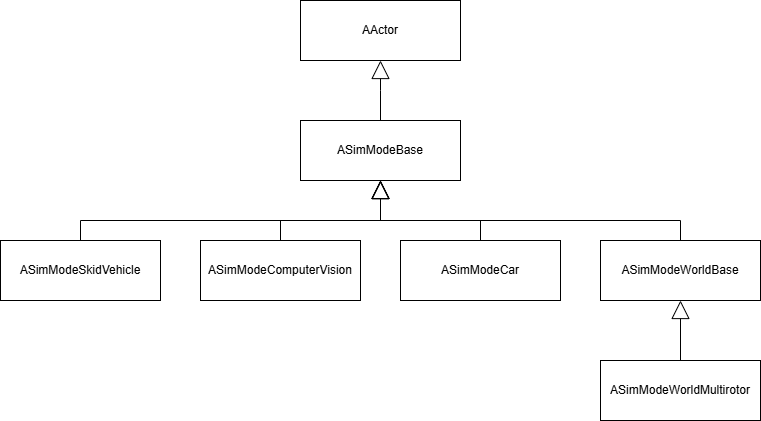
\includegraphics[width=0.7\textwidth]{graphics/simmode_hierarchy.png}
    \caption{\small UML Class Hierarchy for Cosys-AirSim Simulation Modes.}
    \label{fig:simmode_hierarchy}
\end{figure}
\noindent
The initialization process and interaction between the Unreal Engine and the AirSim plugin are illustrated in Figure \ref{fig:airsim_startup}.
\begin{figure}[H]
    \centering
    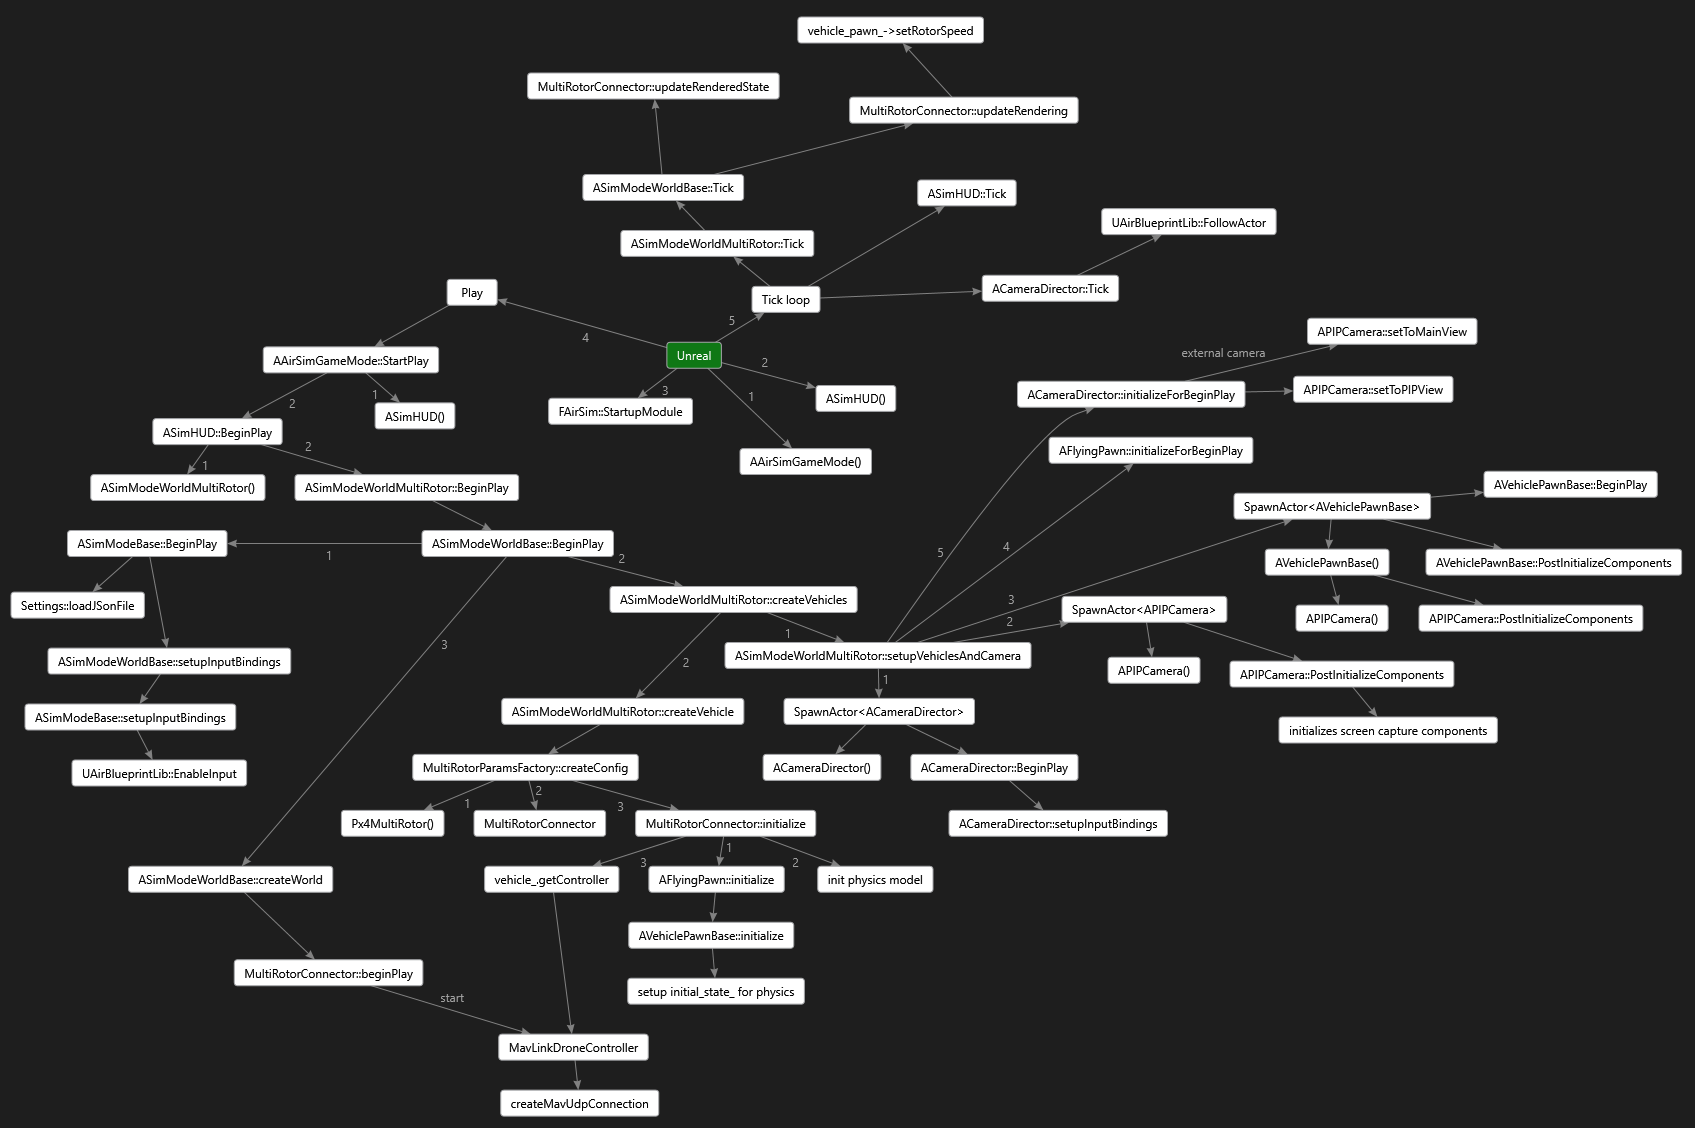
\includegraphics[width=0.7\textwidth]{graphics/airsim_startup.png}
    \caption{\small AirSim loading and invocation by Unreal Engine from the \href{https://airsim-fork.readthedocs.io/en/docs/code_structure.html}{official documentation}.}
    \label{fig:airsim_startup}
\end{figure}

\subsubsection{The Simulation API Bridge}
\noindent
This critical layer manages the bidirectional data flow between the core library and the rendering engine.

\begin{description}
    \item[\texttt{PawnSimApi}:] The primary mediator.  It subscribes to \texttt{pawn\_events} to catch Unreal collisions and frame ticks, while simultaneously implementing the \texttt{VehicleSimApiBase} from AirLib to update the vehicle's 3D transform (position and orientation) based on physics calculations.
    \item[Vehicle-Specific APIs:] Classes like \texttt{CarSimApi} and \texttt{MultirotorSimApi} extend  the base functionality to handle unique actuators, such as wheel rotation, suspension compression, or rotor blur effects, ensuring the visual representation matches the internal physical state.
\end{description}
